\documentclass{extbook}[14pt]
\usepackage{multicol, enumerate, enumitem, hyperref, color, soul, setspace, parskip, fancyhdr, amssymb, amsthm, amsmath, latexsym, units, mathtools}
\everymath{\displaystyle}
\usepackage[headsep=0.5cm,headheight=0cm, left=1 in,right= 1 in,top= 1 in,bottom= 1 in]{geometry}
\usepackage{dashrule}  % Package to use the command below to create lines between items
\newcommand{\litem}[1]{\item #1

\rule{\textwidth}{0.4pt}}
\pagestyle{fancy}
\lhead{}
\chead{Answer Key for Progress Quiz 9 Version A}
\rhead{}
\lfoot{9541-5764}
\cfoot{}
\rfoot{Summer C 2021}
\begin{document}
\textbf{This key should allow you to understand why you choose the option you did (beyond just getting a question right or wrong). \href{https://xronos.clas.ufl.edu/mac1105spring2020/courseDescriptionAndMisc/Exams/LearningFromResults}{More instructions on how to use this key can be found here}.}

\textbf{If you have a suggestion to make the keys better, \href{https://forms.gle/CZkbZmPbC9XALEE88}{please fill out the short survey here}.}

\textit{Note: This key is auto-generated and may contain issues and/or errors. The keys are reviewed after each exam to ensure grading is done accurately. If there are issues (like duplicate options), they are noted in the offline gradebook. The keys are a work-in-progress to give students as many resources to improve as possible.}

\rule{\textwidth}{0.4pt}

\begin{enumerate}\litem{
Construct the lowest-degree polynomial given the zeros below. Then, choose the intervals that contain the coefficients of the polynomial in the form $ax^3+bx^2+cx+d$.
\[ \frac{-3}{4}, \frac{7}{4}, \text{ and } \frac{1}{5} \]The solution is \( 80x^{3} -96 x^{2} -89 x + 21 \), which is option C.\begin{enumerate}[label=\Alph*.]
\item \( a \in [71, 88], b \in [-99, -95], c \in [-89, -81], \text{ and } d \in [-25, -15] \)

$80x^{3} -96 x^{2} -89 x -21$, which corresponds to multiplying everything correctly except the constant term.
\item \( a \in [71, 88], b \in [-222, -215], c \in [143, 147], \text{ and } d \in [-25, -15] \)

$80x^{3} -216 x^{2} +145 x -21$, which corresponds to multiplying out $(4x -3)(4x -7)(5x -1)$.
\item \( a \in [71, 88], b \in [-99, -95], c \in [-89, -81], \text{ and } d \in [16, 31] \)

* $80x^{3} -96 x^{2} -89 x + 21$, which is the correct option.
\item \( a \in [71, 88], b \in [57, 67], c \in [-121, -119], \text{ and } d \in [16, 31] \)

$80x^{3} +64 x^{2} -121 x + 21$, which corresponds to multiplying out $(4x -3)(4x + 7)(5x -1)$.
\item \( a \in [71, 88], b \in [94, 102], c \in [-89, -81], \text{ and } d \in [-25, -15] \)

$80x^{3} +96 x^{2} -89 x -21$, which corresponds to multiplying out $(4x -3)(4x + 7)(5x + 1)$.
\end{enumerate}

\textbf{General Comment:} To construct the lowest-degree polynomial, you want to multiply out $(4x + 3)(4x -7)(5x -1)$
}
\litem{
Describe the end behavior of the polynomial below.
\[ f(x) = 7(x - 7)^{4}(x + 7)^{7}(x - 3)^{2}(x + 3)^{2} \]The solution is the graph below, which is option D.
    \begin{center}
        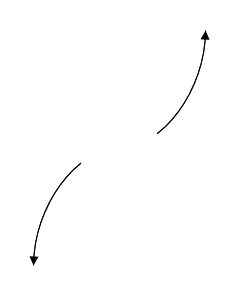
\includegraphics[width=0.3\textwidth]{../Figures/polyEndBehaviorCopyDA.png}
    \end{center}\begin{enumerate}[label=\Alph*.]
\begin{multicols}{2}
\item 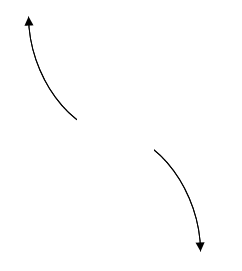
\includegraphics[width = 0.3\textwidth]{../Figures/polyEndBehaviorCopyAA.png}
\item 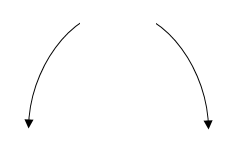
\includegraphics[width = 0.3\textwidth]{../Figures/polyEndBehaviorCopyBA.png}
\item 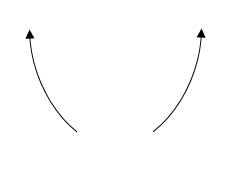
\includegraphics[width = 0.3\textwidth]{../Figures/polyEndBehaviorCopyCA.png}
\item 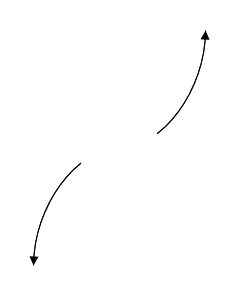
\includegraphics[width = 0.3\textwidth]{../Figures/polyEndBehaviorCopyDA.png}
\end{multicols}\item None of the above.\end{enumerate}
\textbf{General Comment:} Remember that end behavior is determined by the leading coefficient AND whether the \textbf{sum} of the multiplicities is positive or negative.
}
\litem{
Construct the lowest-degree polynomial given the zeros below. Then, choose the intervals that contain the coefficients of the polynomial in the form $x^3+bx^2+cx+d$.
\[ 5 - 4 i \text{ and } -4 \]The solution is \( x^{3} -6 x^{2} +x + 164 \), which is option C.\begin{enumerate}[label=\Alph*.]
\item \( b \in [3, 20], c \in [-0.68, 1.9], \text{ and } d \in [-168, -161] \)

$x^{3} +6 x^{2} +x -164$, which corresponds to multiplying out $(x-(5 - 4 i))(x-(5 + 4 i))(x -4)$.
\item \( b \in [-1, 4], c \in [5.04, 8.21], \text{ and } d \in [16, 23] \)

$x^{3} + x^{2} +8 x + 16$, which corresponds to multiplying out $(x + 4)(x + 4)$.
\item \( b \in [-6, -4], c \in [-0.68, 1.9], \text{ and } d \in [164, 166] \)

* $x^{3} -6 x^{2} +x + 164$, which is the correct option.
\item \( b \in [-1, 4], c \in [-1.45, 0.42], \text{ and } d \in [-20, -17] \)

$x^{3} + x^{2} -x -20$, which corresponds to multiplying out $(x -5)(x + 4)$.
\item \( \text{None of the above.} \)

This corresponds to making an unanticipated error or not understanding how to use nonreal complex numbers to create the lowest-degree polynomial. If you chose this and are not sure what you did wrong, please contact the coordinator for help.
\end{enumerate}

\textbf{General Comment:} Remember that the conjugate of $a+bi$ is $a-bi$. Since these zeros always come in pairs, we need to multiply out $(x-(5 - 4 i))(x-(5 + 4 i))(x-(-4))$.
}
\litem{
Which of the following equations \textit{could} be of the graph presented below?

\begin{center}
    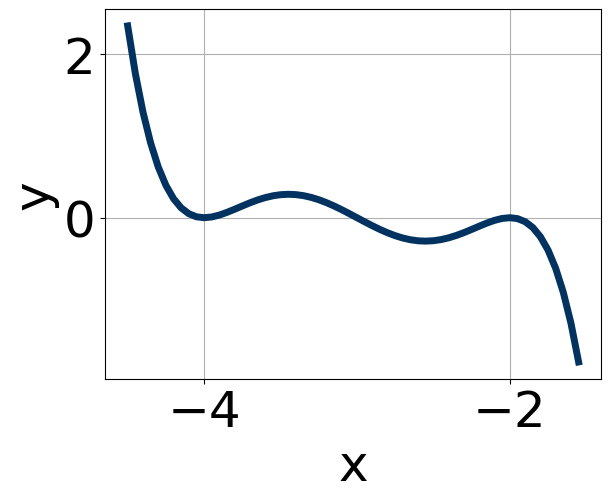
\includegraphics[width=0.5\textwidth]{../Figures/polyGraphToFunctionCopyA.png}
\end{center}


The solution is \( -6(x + 2)^{10} (x + 4)^{6} (x + 3)^{5} \), which is option D.\begin{enumerate}[label=\Alph*.]
\item \( -13(x + 2)^{10} (x + 4)^{7} (x + 3)^{6} \)

The factor $(x + 4)$ should have an even power and the factor $(x + 3)$ should have an odd power.
\item \( 18(x + 2)^{10} (x + 4)^{6} (x + 3)^{10} \)

The factor $(x + 3)$ should have an odd power and the leading coefficient should be the opposite sign.
\item \( 16(x + 2)^{4} (x + 4)^{4} (x + 3)^{5} \)

This corresponds to the leading coefficient being the opposite value than it should be.
\item \( -6(x + 2)^{10} (x + 4)^{6} (x + 3)^{5} \)

* This is the correct option.
\item \( -15(x + 2)^{6} (x + 4)^{7} (x + 3)^{11} \)

The factor $(x + 4)$ should have an even power.
\end{enumerate}

\textbf{General Comment:} General Comments: Draw the x-axis to determine which zeros are touching (and so have even multiplicity) or cross (and have odd multiplicity).
}
\litem{
Describe the zero behavior of the zero $x = -8$ of the polynomial below.
\[ f(x) = 6(x + 7)^{3}(x - 7)^{2}(x - 8)^{5}(x + 8)^{4} \]The solution is the graph below, which is option C.
    \begin{center}
        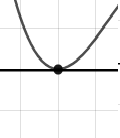
\includegraphics[width=0.3\textwidth]{../Figures/polyZeroBehaviorCopyCA.png}
    \end{center}\begin{enumerate}[label=\Alph*.]
\begin{multicols}{2}
\item 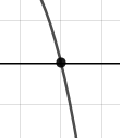
\includegraphics[width = 0.3\textwidth]{../Figures/polyZeroBehaviorCopyAA.png}
\item 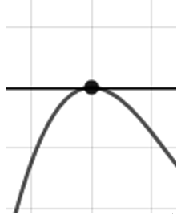
\includegraphics[width = 0.3\textwidth]{../Figures/polyZeroBehaviorCopyBA.png}
\item 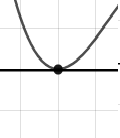
\includegraphics[width = 0.3\textwidth]{../Figures/polyZeroBehaviorCopyCA.png}
\item 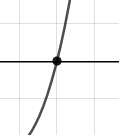
\includegraphics[width = 0.3\textwidth]{../Figures/polyZeroBehaviorCopyDA.png}
\end{multicols}\item None of the above.\end{enumerate}
\textbf{General Comment:} You will need to sketch the entire graph, then zoom in on the zero the question asks about.
}
\litem{
Describe the zero behavior of the zero $x = -9$ of the polynomial below.
\[ f(x) = -2(x + 9)^{6}(x - 9)^{9}(x - 8)^{2}(x + 8)^{5} \]The solution is the graph below, which is option B.
    \begin{center}
        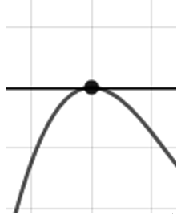
\includegraphics[width=0.3\textwidth]{../Figures/polyZeroBehaviorBA.png}
    \end{center}\begin{enumerate}[label=\Alph*.]
\begin{multicols}{2}
\item 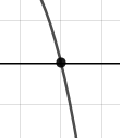
\includegraphics[width = 0.3\textwidth]{../Figures/polyZeroBehaviorAA.png}
\item 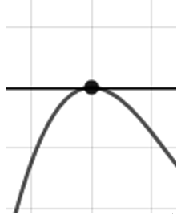
\includegraphics[width = 0.3\textwidth]{../Figures/polyZeroBehaviorBA.png}
\item 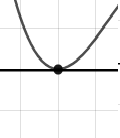
\includegraphics[width = 0.3\textwidth]{../Figures/polyZeroBehaviorCA.png}
\item 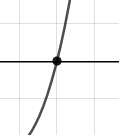
\includegraphics[width = 0.3\textwidth]{../Figures/polyZeroBehaviorDA.png}
\end{multicols}\item None of the above.\end{enumerate}
\textbf{General Comment:} You will need to sketch the entire graph, then zoom in on the zero the question asks about.
}
\litem{
Describe the end behavior of the polynomial below.
\[ f(x) = -4(x - 2)^{3}(x + 2)^{4}(x - 9)^{5}(x + 9)^{5} \]The solution is the graph below, which is option A.
    \begin{center}
        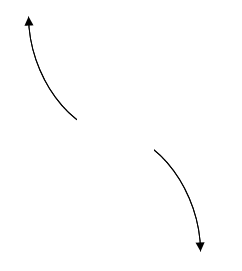
\includegraphics[width=0.3\textwidth]{../Figures/polyEndBehaviorAA.png}
    \end{center}\begin{enumerate}[label=\Alph*.]
\begin{multicols}{2}
\item 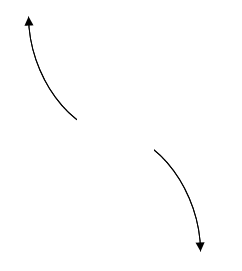
\includegraphics[width = 0.3\textwidth]{../Figures/polyEndBehaviorAA.png}
\item 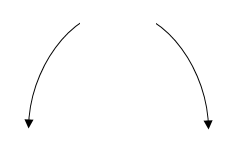
\includegraphics[width = 0.3\textwidth]{../Figures/polyEndBehaviorBA.png}
\item 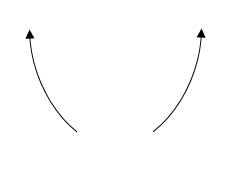
\includegraphics[width = 0.3\textwidth]{../Figures/polyEndBehaviorCA.png}
\item 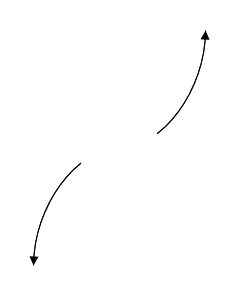
\includegraphics[width = 0.3\textwidth]{../Figures/polyEndBehaviorDA.png}
\end{multicols}\item None of the above.\end{enumerate}
\textbf{General Comment:} Remember that end behavior is determined by the leading coefficient AND whether the \textbf{sum} of the multiplicities is positive or negative.
}
\litem{
Construct the lowest-degree polynomial given the zeros below. Then, choose the intervals that contain the coefficients of the polynomial in the form $x^3+bx^2+cx+d$.
\[ -3 + 2 i \text{ and } 1 \]The solution is \( x^{3} +5 x^{2} +7 x -13 \), which is option B.\begin{enumerate}[label=\Alph*.]
\item \( b \in [-6.2, -2.7], c \in [7, 14], \text{ and } d \in [10, 14] \)

$x^{3} -5 x^{2} +7 x + 13$, which corresponds to multiplying out $(x-(-3 + 2 i))(x-(-3 - 2 i))(x + 1)$.
\item \( b \in [1.3, 5.6], c \in [7, 14], \text{ and } d \in [-16, -7] \)

* $x^{3} +5 x^{2} +7 x -13$, which is the correct option.
\item \( b \in [-0.3, 3.3], c \in [-2, 3], \text{ and } d \in [-5, 0] \)

$x^{3} + x^{2} +2 x -3$, which corresponds to multiplying out $(x + 3)(x -1)$.
\item \( b \in [-0.3, 3.3], c \in [-6, -1], \text{ and } d \in [0, 3] \)

$x^{3} + x^{2} -3 x + 2$, which corresponds to multiplying out $(x -2)(x -1)$.
\item \( \text{None of the above.} \)

This corresponds to making an unanticipated error or not understanding how to use nonreal complex numbers to create the lowest-degree polynomial. If you chose this and are not sure what you did wrong, please contact the coordinator for help.
\end{enumerate}

\textbf{General Comment:} Remember that the conjugate of $a+bi$ is $a-bi$. Since these zeros always come in pairs, we need to multiply out $(x-(-3 + 2 i))(x-(-3 - 2 i))(x-(1))$.
}
\litem{
Construct the lowest-degree polynomial given the zeros below. Then, choose the intervals that contain the coefficients of the polynomial in the form $ax^3+bx^2+cx+d$.
\[ \frac{-5}{4}, \frac{-3}{4}, \text{ and } 5 \]The solution is \( 16x^{3} -48 x^{2} -145 x -75 \), which is option C.\begin{enumerate}[label=\Alph*.]
\item \( a \in [15, 19], b \in [42, 52], c \in [-151, -140], \text{ and } d \in [68, 80] \)

$16x^{3} +48 x^{2} -145 x + 75$, which corresponds to multiplying out $(4x -5)(4x -3)(x + 5)$.
\item \( a \in [15, 19], b \in [-48, -41], c \in [-151, -140], \text{ and } d \in [68, 80] \)

$16x^{3} -48 x^{2} -145 x + 75$, which corresponds to multiplying everything correctly except the constant term.
\item \( a \in [15, 19], b \in [-48, -41], c \in [-151, -140], \text{ and } d \in [-76, -69] \)

* $16x^{3} -48 x^{2} -145 x -75$, which is the correct option.
\item \( a \in [15, 19], b \in [-94, -79], c \in [23, 34], \text{ and } d \in [68, 80] \)

$16x^{3} -88 x^{2} +25 x + 75$, which corresponds to multiplying out $(4x -5)(4x + 3)(x -5)$.
\item \( a \in [15, 19], b \in [-119, -111], c \in [173, 179], \text{ and } d \in [-76, -69] \)

$16x^{3} -112 x^{2} +175 x -75$, which corresponds to multiplying out $(4x -5)(4x -3)(x -5)$.
\end{enumerate}

\textbf{General Comment:} To construct the lowest-degree polynomial, you want to multiply out $(4x + 5)(4x + 3)(x -5)$
}
\litem{
Which of the following equations \textit{could} be of the graph presented below?

\begin{center}
    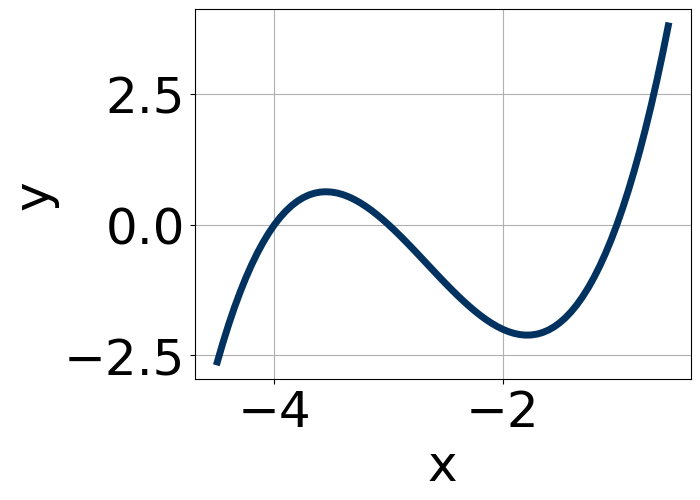
\includegraphics[width=0.5\textwidth]{../Figures/polyGraphToFunctionA.png}
\end{center}


The solution is \( 10(x + 1)^{11} (x + 3)^{7} (x + 4)^{11} \), which is option C.\begin{enumerate}[label=\Alph*.]
\item \( 5(x + 1)^{8} (x + 3)^{4} (x + 4)^{5} \)

The factors $-1$ and $-3$ have have been odd power.
\item \( -17(x + 1)^{4} (x + 3)^{5} (x + 4)^{5} \)

The factor $(x + 1)$ should have an odd power and the leading coefficient should be the opposite sign.
\item \( 10(x + 1)^{11} (x + 3)^{7} (x + 4)^{11} \)

* This is the correct option.
\item \( 5(x + 1)^{4} (x + 3)^{11} (x + 4)^{11} \)

The factor $-1$ should have been an odd power.
\item \( -9(x + 1)^{7} (x + 3)^{11} (x + 4)^{9} \)

This corresponds to the leading coefficient being the opposite value than it should be.
\end{enumerate}

\textbf{General Comment:} General Comments: Draw the x-axis to determine which zeros are touching (and so have even multiplicity) or cross (and have odd multiplicity).
}
\end{enumerate}

\end{document}